\apendice{Plan de Proyecto Software}

\renewcommand{\arraystretch}{1.4}
\section{Introducción}

A continuación, se redacta la planificación llevada a cabo para desarrollar este proyecto. En primer lugar, a nivel temporal, se especifican las etapas de trabajo en forma de tareas. A nivel económico, se estiman los costes totales de cada parte implicada. Por último, a nivel legal, se indican las especificaciones requeridas para su desempeño.

\section{Planificación temporal}
Para la planificación temporal, se ha optado por utilizar un diagrama de Gantt, ya que el presente trabajo tiene un recorrido lineal y progresivo, no iterativo, y se ha realizado siguiendo un enfoque por fases de desarrollo técnico y de forma cronológica. 

Como paso previo a dicho diagrama, en la Tabla~\ref{tab:milestones} se recogen los principales hitos alcanzados durante el proyecto, junto con su correspondencia con las issues cerradas en el repositorio de GitHub\footnote{Link al repositorio de GitHub: \href{https://github.com/ElenaRuizMoreno/TFG-Elena-Ruiz/}{TFG - Elena Ruiz}}.

\vspace{0.3cm}
\begin{table}[H]
\centering
\renewcommand{\arraystretch}{1.1} % Reducido de 1.5 a 1.1
\begin{tabularx}{\textwidth}{|l|X|X|}
\hline
\textbf{Milestone} & \textbf{Descripción} & \textbf{Issues asociadas} \\
\hline
1 & Recopilación de información bibliográfica & \#1 \\
\hline
2 & Redacción de memoria con Latex & 
\#2, \#7, \#11, \#24, \#25, \#26, \#27, \#28, \#29 \\
\hline
3 & Configuración inicial del entorno de desarrollo y pruebas del pulsioxímetro & 
\#3, \#4, \#5, \#6 \\
\hline
4 & Análisis de datos crudos del sensor & 
\#8, \#9, \#10 \\
\hline
5 & Validación e implementación final de los algoritmos & \#12, \#14 \\
\hline
6 & Redacción de los anexos con Latex & 
\#13, \#15, \#18, \#19, \#20, \#21, \#22, \#23 \\
\hline
7 & Organización final del repositorio & 
\#16, \#17 \\
\hline
\end{tabularx}
\caption{Resumen de milestones del proyecto y issues asociadas. \textit{Elaboración propia.}}
\label{tab:milestones}
\end{table}


A continuación, se enumeran las tareas completadas hasta la fecha, con una breve descripción de cada una. 
\vspace{0.3cm}

\textbf{Recopilación de información bibliográfica}

Issue \textit{\#1 Búsqueda Bibliográfica.}

Periodo: 30/10/2024 - 10/04/2025.


\begin{itemize}
    \item Investigación sobre el funcionamiento de un pulsioxímetro y estado del arte de trabajos relacionados.
    \item Búsqueda de artículos y documentación sobre estimación de frecuencia cardíaca y saturación de oxígeno a partir de señales PPG.
\end{itemize}

\textbf{Configuración inicial del entorno de desarrollo y pruebas del pulsioxímetro}

Issue \textit{\#3 Seguimiento de comunicación y definición del alcance del pulsioxímetro.}

Periodo: 18/12/2024 - 20/02/2025.

\begin{itemize}
    \item Contacto con la organización para plantear el objetivo principal.
    \item Organización del envío y revisión del material proporcionado por la ONG \href{https://medicalopenworld.org/}{Medicina Abierta al Mundo}.
    \item Definición del alcance del pulsioxímetro en el sistema de incubadora y análisis del hardware disponible.
\end{itemize}

Issue \textit{\#4 Preparación del hardware: recepción y primeros ajustes.}

Periodo: 30/01/2025 - 05/03/2025.

Reuniones presenciales en el laboratorio para realizar pruebas de comunicación y validación del montaje de hardware.

\vspace{0.3cm}

Issue \textit{\#5 Instalación y configuración de los drivers del programador.}

Periodo: 11/02/2025 - 05/03/2025.

\begin{itemize}
    \item Instalación y configuración del entorno de desarrollo (Visual Studio Code + PlatformIO).
    \item Instalación de drivers necesarios para la conexión con la PCB.
\end{itemize}


Issue \textit{\#6 Captura y registro de datos crudos del sensor.}

Periodo: 02/03/2025 – 21/04/2025.

\begin{itemize}
    \item Desarrollo de varias versiones de una función concreta del firmware para registrar datos en un determinado periodo y frecuencia óptimos para su posterior análisis.
    \item Implementación de un script en Python para guardar datos del pulsioxímetro en formato CSV con inclusión de encabezados y una referencia al tiempo en ms.
    \item Sesiones de captura de datos con distintos resultados hasta conseguir los suficientes registros con la mejor calidad posible.
\end{itemize}

\textbf{Análisis de datos crudos del sensor.}

Issue \textit{\#8 Análisis de datos: Visualización de señales y siguientes pasos.}

Periodo: 10/03/2025 - 07/04/2025.

\begin{itemize}
    \item Lectura y visualización de los registros obtenidos.
    \item Clasificación de señales por calidad, y preparación para análisis cuantitativo.
\end{itemize}


Issue \textit{\#9 Cálculo de la frecuencia cardíaca a partir de los datos crudos del sensor.}

Periodo: 17/03/2025 - 05/04/2025.

\begin{itemize}
    \item Búsqueda de artículos y métodos relacionados con la estimación del valor de frecuencia cardíaca a partir de señales PPG procedentes de un pulsioxímetro.
    \item Implementación de diferentes métodos para detección de picos y cálculo de frecuencia cardíaca.
\end{itemize}


Issue \textit{\#10 Cálculo del valor de SpO$_2$ a partir de los datos crudos del sensor.}

Periodo: 07/04/2025 – 09/05/2025.

\begin{itemize}
    \item Documentación acerca de los principales métodos del cálculo de la saturación de oxígeno.
    \item Implementación de distintos algoritmos de cálculo (Ratio of Ratios, tabla LUT) en Python combinados con diferentes procesamientos.
\end{itemize}


\textbf{Validación e implementación final de los algoritmos}

Issue \textit{\#12 Análisis y optimización del tiempo de cómputo de los algoritmos de pulsioximetría.}

Periodo: 24/04/2025 - 13/05/2025.

Estudio del tiempo de cómputo de los algoritmos que mejores resultados ofrecían.

\vspace{0.3cm}

Issue \textit{\#14 Implementación en firmware de los algoritmos validados.}

Periodo: 09/05/2025 - 25/05/2025.

\begin{itemize}
    \item Adaptación del código Python a C++ para su inclusión en el firmware del ESP32.
    \item Pruebas con datos reales en entorno embebido.
\end{itemize}

\textbf{Redacción de la memoria con Latex}

\textit{\#2 Conceptos teóricos.}

Periodo: 18/01/2025 - 25/05/2025.

\begin{itemize}
    \item Desarrollo de los conceptos teóricos en la memoria teórica, que sirvió tanto para empezar a estructurar la memoria, como para dejar claros los fundamentos teóricos que definen el proyecto y así facilitar su comprensión.
\end{itemize}

Issue \textit{\#7 Comprensión y configuración de LaTeX para la memoria y anexos.}

Periodo: 05/03/2025 – 10/05/2025.

\begin{itemize}
    \item Descarga y adaptación de la plantilla oficial del TFG del grado de ingeniería de la salud.
    \item Comprensión básica de LaTeX, estructura de documentos, gestión de bibliografía y compilación.
\end{itemize}

Issue \textit{\#11 Redacción de la metodología.}

Periodo: 08/04/2025 – 02/06/2025.

\begin{itemize}
    \item Descripción de los datos utilizados a lo largo del proyecto, así como el proceso de adquisición de los mismos.
    \item Explicación de las herramientas hardware y software utilizadas.
    \item Documentación detallada del procedimiento experimental, filtros aplicados, y algoritmos utilizados.
\end{itemize}

Issue \textit{\#24 Resultados.}

Periodo: 03/06/2025 – 08/06/2025.

\begin{itemize}
    \item Resumen de los principales resultados obtenidos y breve explicación de los mismos a través de tablas de valores y gráficos demostrativos.
    \item Inclusión de capturas de pantalla del firmware que demuestran el funcionamiento del sistema, además de la referencia a un pequeño vídeo demostrativo de la solución desarollada en tiempo real.
\end{itemize}

Issue \textit{\#25 Conlcusiones.}

Periodo: 03/06/2025 – 08/06/2025

\begin{itemize}
    \item Presentación de las conclusiones obtenidas, relacionándolas con los objetivos del proyecto.
    \item Discusión de los resultados enfrentándolos a otros proyectos relacionados ya mencionados con anterioridad.
\end{itemize}

Issue \textit{\#26 Líneas de trabajo futuras.}

Periodo: 03/06/2025 – 08/06/2025.

Presentación de las principales líneas de trabajo que se consideran oportunas para continuar en un futuro con el sistema desarrollado y mejorarlo.

\vspace{0.3cm}

Issue \textit{\#27 Resumen.}

Periodo: 04/06/2025 – 08/06/2025.

\begin{itemize}
    \item Elaboración del resumen del trabajo sintentizando objetivos principales, metodología, resultados y conclusiones.
    \item Enumeración de las palabras clave relacionadas con el trabajo realizado.
\end{itemize}

Issue \textit{\#28 Introducción.}

Periodo: 05/06/2025 – 08/06/2025

Contextualización del problema a resolver por el sistema que se ha elaborado y breve explicación de como se ha abordado.

\vspace{0.3cm}

Issue \textit{\#29 Objetivos.}

Periodo estimado: 05/06/2025 – 08/06/2025

Enumeración del objetivo principal del proyecto planteado, objetivos personales y funcionales del sistema.

\newpage

\textbf{Organización final del repositorio}

Issue \textit{\#16 Clasificación de notebooks por validez de los métodos.}

Periodo: 13/05/2025 – 25/05/2025

\begin{itemize}
    \item Revisión de los notebooks desarrollados durante el análisis de frecuencia cardiaca y SpO$_2$.
    \item Evaluación de la validez de cada uno según señal de entrada, métricas, código y optimización.
    \item Eliminación o documentación de los notebooks no válidos, para evitar confusión en fases finales.
\end{itemize}

Issue \textit{\#17 Revisión y limpieza de notebooks definitivos.}

Periodo estimado: 13/05/2025 – 25/05/2025

\begin{itemize}
    \item Unificación del estilo y estructura de todos los notebooks definitivos del proyecto.
    \item Inclusión de comentarios explicativos para comprender lo que hace el código.
\end{itemize}

\textbf{Redacción de los anexos con Latex}

Issue \textit{\#13 Anexo A: Planificación del Proyecto.}

Periodo estimado: 24/05/2025 – 08/06/2025

\begin{itemize}
    \item Redacción del anexo que detalla la planificación temporal, económica y legal del proyecto.
    \item Relación entre las tareas descritas y las issues del repositorio de GitHub.
\end{itemize}

Issue \textit{\#15 Anexo D: Descripción y adquisición de los datos.}

Periodo estimado: 09/05/2025 – 08/06/2025

\begin{itemize}
    \item Documentación del procedimiento de captura y preprocesamiento de señales del pulsioxímetro.
    \item Explicación del formato de los ficheros CSV y descripción de la naturaleza de la señal registrada.
\end{itemize}

Issue \textit{\#18 Redacción del Anexo B: Documentación de Usuario.}

Periodo estimado: 25/05/2025 – 08/06/2025

\begin{itemize}
    \item Inclusión de requisitos software y hardware del sistema completo.
    \item Manual paso a paso para la instalación, ejecución y uso por parte de usuarios no técnicos.
\end{itemize}

Issue \textit{\#19 Redacción del Anexo C: Manual del Desarrollador.}

Periodo estimado: 25/05/2025 – 08/06/2025

\begin{itemize}
    \item Explicación de estructura de carpetas, herramientas utilizadas y dependencias.
    \item Documentación técnica para futuros desarrolladores del sistema.
    \item Instrucciones para compilar, modificar y validar el firmware y los scripts de análisis.
\end{itemize}

Issue \textit{\#20 Redacción del Anexo E: Especificación de Diseño.}

Periodo estimado: 25/05/2025 – 08/06/2025

\begin{itemize}
    \item Descripción del punto de partida del proyecto.
    \item Inclusión de diagramas de bloques, interfaz sensor-microcontrolador y resumen del algoritmo.
\end{itemize}

Issue \textit{\#21 Redacción del Anexo F: Especificación de Requisitos.}

Periodo estimado: 02/06/2025 – 08/06/2025

Adaptación del anexo a la naturaleza del proyecto y descripción del caso de uso principal.


Issue \textit{\#22 Redacción del Anexo G: Estudio experimental.}

Periodo estimado: 02/06/2025 – 08/06/2025

\begin{itemize}
    \item Descripción cronológica de todo lo realizado en forma de cuaderno de trabajo, incluyendo resultados negativos.
    \item Enumeración de los parámetros utilizados en los algoritmos.
\end{itemize}

Issue \textit{\#23 Redacción del Anexo H: Anexo de sostenibilización circular.}

Periodo estimado: 02/06/2025 – 08/06/2025

Identificación de los principales objetivos de desarrollo sostenible a los que se adhiere el proyecto realizado y explicar el por qué.

\begin{figure}[H]
    \centering
    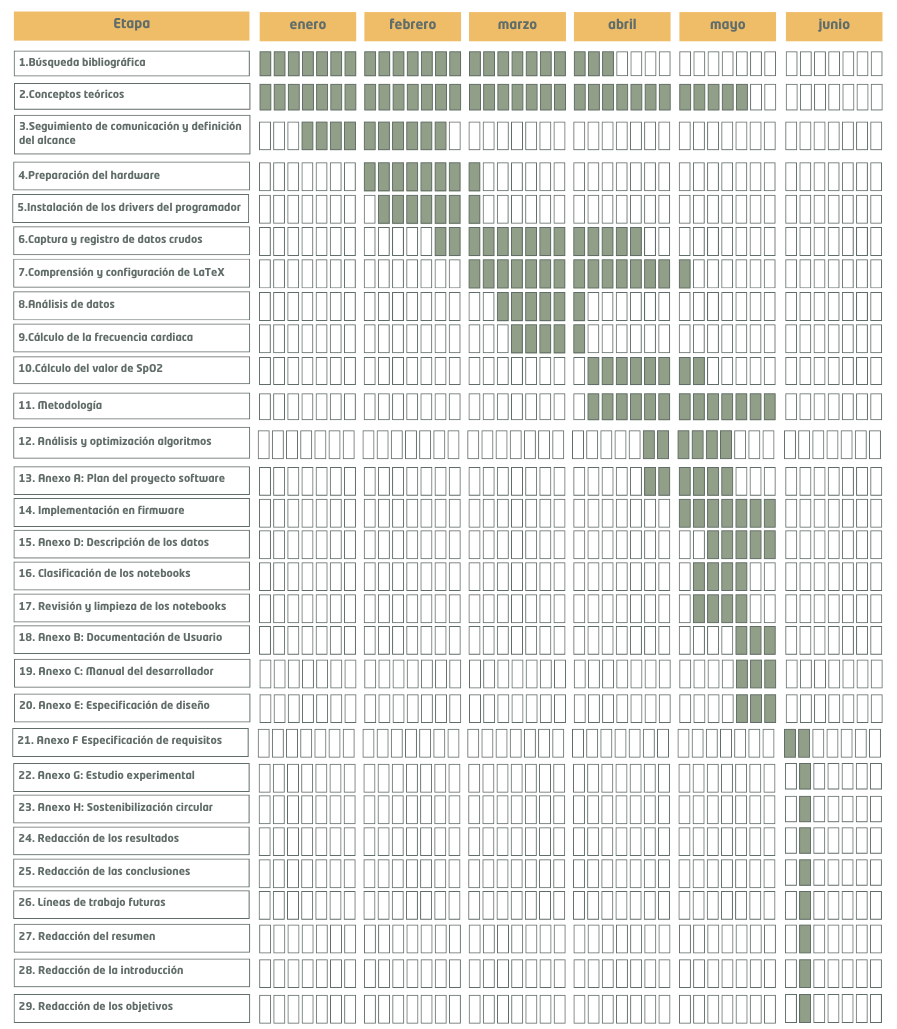
\includegraphics[width=0.9\linewidth]{img/DIAGRAMAGANTT.png}
    \caption{Representación de la planificación temporal seguida según las issues a partir de un diagrama de Gantt.\textit{ Elaboración propia.}}
    \label{fig:DIAGRAMAGANTT}
\end{figure}

\section{Planificación económica}
Se indican en este apartado los costes tanto personales como de
materiales, hardware y software necesarios.

\subsection{Costes personales}

Este proyecto se ha llevado a cabo completamente como parte de un Trabajo de Fin de Grado sin recibir compensación económica directa por ello. Sin embargo, para poder reflejar el valor técnico y hacer una comparación realista con su desarrollo en un entorno profesional, se ha calculado el coste equivalente al tiempo de trabajo que se ha invertido.

Para estimar este coste, se ha tomado como referencia el salario bruto medio de entrada en el mercado laboral para un perfil de ingeniería recién graduado en España, situado en torno a los 25.000 € brutos anuales a jornada completa \cite{ufv:salario}. Esto equivale a un salario mensual bruto de aproximadamente 1.763 € (en 14 pagas), con un salario neto estimado en torno a 1.500 € tras aplicar las deducciones correspondientes.

Debido a que para el desarrollo de este proyecto se ha trabajado una media de 4 horas diarias, distribuidas en 5 días a la semana, se considera equivalente a una jornada parcial (media jornada) típica de un ingeniero junior.

Partiendo de un salario bruto anual de 25.000 € para una jornada completa, el salario bruto anual estimado para una jornada parcial equivalente (media jornada) se reduce a la mitad:

\[
\frac{25.000 \text{€}}{2} = \textbf{12.500 €}
\]

Considerando una jornada parcial de 4 horas al día durante 5 días a la semana, teniendo 42 semanas laborales al año:

\[
4\,\text{h/día} \times 5\,\text{días/sem} \times 42\,\text{sem} = \textbf{840\,h/año}
\]

De ahí se obtiene el coste por hora bruto:

\[
\frac{12.500 \text{€}}{840\,h} = \textbf{14{,}88 €/h}
\]

Aplicando una retención del 16\% (factor 0,84) para IRPF y cotizaciones sociales, se obtiene el coste por hora neto:

\[
14{,}88 \text{€} \times 0{,}84 = \textbf{12{,}50 €/h}
\]


\begin{table}[H]
\centering
\begin{tabular}{|l|c|}
\hline
\textbf{Concepto} & \textbf{Valor} \\
\hline
Salario bruto anual estimado (media jornada) & 12.500 € \\
Horas anuales estimadas (media jornada) & 840 h \\
Coste por hora (bruto) & 14{,}88 €/h \\
Coste por hora (neto) & 12{,}5 €/h\\
\hline
\end{tabular}
\caption{Estimación del coste por hora a media jornada de un ingeniero recién graduado.}
\label{tab:coste_hora}
\end{table}

A partir del seguimiento real del trabajo realizado durante el proyecto, se estima una dedicación total de aproximadamente 480 horas efectivas distribuidas a lo largo de seis meses. Esta estimación contempla tareas técnicas, adquisición de señales, validación de algoritmos y redacción de la documentación. No se han incluido en este cómputo las actividades relacionadas con el desarrollo previo de la placa base y el firmware completo de la incubadora, ya que se ha partido de este material ya desarrollado por la organización.

Aplicando el coste por hora neto estimado, el coste personal total equivalente asciende a:

\[
480 \, \text{h} \times 12,5\, \frac{\text{€}}{\text{h}} = \textbf{6.000\,€}
\]


\subsection{Costes de herramientas utilizadas}

Durante el proyecto se ha utilizado, por una parte, equipamiento propio y por otra, material prestado de la ONG Medicina Abierta al Mundo.  A continuación, se detallan los costes amortizados de dichos recursos, suponiendo una vida útil de 4 años y una utilización de 6 meses.

Dado que se trata de un desarrollo centrado en software, la herramienta principal empleada ha sido un ordenador portátil:

\begin{table}[H]
\centering
\begin{tabular}{|l|c|c|}
\hline
\textbf{Concepto} & \textbf{Precio total} & \textbf{Amortización 6 meses} \\
\hline
Ordenador portátil HP Core i5 & 600 €\footnotemark[1] & 75 € \\
Licencia Office 365 anual & 99 €\footnotemark[2] & 49,5 € \\
\hline
\textbf{Total} & 699 € & \textbf{124,5 €} \\
\hline
\end{tabular}
\caption{Costes de las herramientas personales amortizados a 6 meses.}
\label{tab:costes-amortizados}
\end{table}


\footnotetext[1]{Precio de referencia de la gama HP Core i5 consultado en la página oficial de HP \cite{hp2024}.}
\footnotetext[2]{En nuestro caso, la licencia Office 365 está cubierta por la Universidad de Burgos, pero en el peor de los casos, el precio de la suscripción a Office 365 personal anual, está disponible en la web de Microsoft \cite{microsoft2024}.}




\subsubsection{Costes de materiales para el prototipo}

El sistema fue validado con un prototipo basado en una PCB que simulaba la incubadora y complementado con electrónica de apoyo  facilitada por la ONG:

\begin{table}[H]
\centering
\begin{tabular}{|l|c|c|}
\hline
\textbf{Elemento} & \textbf{Precio (2025)} & \textbf{Proveedor} \\
\hline
PCBA (Placa electrónica) & 60,00 € & JLCPCB\footnotemark[3] \\
Display táctil 7”         & 40,00 € & Elecrow\footnotemark[4] \\
Fuente alimentación 12V (20A mín.) & 9,00 € & Alibaba\footnotemark[5] \\
Cable microUSB  & 4,78 € & StarTech\footnotemark[6] \\
Sensor UA401-D (pulsioxímetro) & 13,69 € & Alibaba\footnotemark[5] \\
Cable IEC C13 europeo 3 metros & 2,00€ & Alibaba\footnotemark[5] \\
Enchufe CA IEC320 (C14 AC-04) & 2,20€ & AliExpress\footnotemark[7] \\
Placa de desarrollo ESP-Prog & 16,76€ & AliExpress \footnotemark[7] \\
Pulsioxímetro comercial 1 & 12,46 € & Berrcom\footnotemark[8]\\
Pulsioxímetro comercial 2 & 28,99 € & Dr. Senst\footnotemark[9]\\
\hline
\textbf{Total} & \textbf{189,88 €} & \\
\hline
\end{tabular}
\caption{Costes actualizados de los materiales del sistema de pulsioximetría (precios 2025).}
\label{tab:costes_pulsioximetro}
\end{table}

\footnotetext[3]{Consultar aquí \href{https://jlcpcb.com}{JLCPCB}}
\footnotetext[4]{Consultar aquí \href{https://www.elecrow.com}{Elecrow}}
\footnotetext[5]{Consultar aquí \href{https://www.alibaba.com}{Alibaba}}
\footnotetext[6]{Consultar aquí \href{https://www.startech.com/}{StarTech}}
\footnotetext[7]{Consultar aquí \href{https://www.aliexpress.com/}{AliExpress}}
\footnotetext[8]{Consultar aquí \href{https://www.berrcomonline.com}{Berrcom}}
\footnotetext[9]{Consultar aquí \href{https://www.dr-senst.com/}{DrSenst}}



\noindent Los costes de cada componente han sido solicitados al responsable del proyecto, que nos lo ha cedido. 

\subsection{Resumen de costes estimados}

\begin{table}[H]
\centering
\begin{tabular}{|l|c|}
\hline
\textbf{Categoría} & \textbf{Coste } \\
\hline
Coste personal estimado            & 6.000€ \\
Herramientas y software (amortizado) & 124{,}5€ \\
Materiales y hardware del prototipo & 189,88€ \\
\hline
\textbf{Total estimado}             & \textbf{6.314,38€} \\
\hline
\end{tabular}
\caption{Resumen del coste económico del proyecto.}
\label{tab:coste_total}
\end{table}

\noindent Este coste no contempla producción en serie ni certificación sanitaria. Si el sistema se escalase para su implementación real en incubadoras clínicas, sería necesario incorporar gastos de validación normativa, fabricación, I+D adicional y soporte técnico.


\section{Viabilidad legal}

En este apartado se analizan las normativas relacionadas con el uso de datos, la distribución del software, y las posibles exigencias regulatorias si el sistema evolucionara hacia un dispositivo médico integrado en un entorno clínico real. 

\vspace{0.3cm}
\subsection{Uso de datos biomédicos}

Durante el desarrollo del sistema se han utilizado datos de señales ópticas  generadas a partir de pruebas con parámetros fisiológicos propios. En ningún momento se han utilizado datos de pacientes ni información sensible o identificativa. Todos los registros utilizados (valores de pulsioximetría) se almacenaron de forma local y sin vinculación a personas concretas, cumpliendo así con el Reglamento General de Protección de Datos (RGPD, UE 2016/679) y la LOPDGDD española (Ley Orgánica 3/2018).

\begin{itemize}
    \item El \textbf{Reglamento General de Protección de Datos} (\textbf{RGPD}, Reglamento (UE) 2016/679)\cite{rgpd2016}, establece las condiciones legales para el tratamiento de datos personales dentro de la Unión Europea. Aunque este trabajo no implica datos identificativos, se ha respetado el principio de minimización y anonimización exigido por el reglamento.
    
    \item La \textbf{Ley Orgánica 3/2018}, de Protección de Datos Personales y garantía de los derechos digitales (\textbf{LOPDGDD})\cite{lopd2018}, adapta el RGPD al contexto jurídico español e introduce medidas específicas para entornos educativos y de investigación. En este sentido, se cumple con las condiciones que permiten el uso de datos biomédicos anonimizados para fines académicos sin requerir consentimiento explícito, garantizando en todo momento la protección de la privacidad.
\end{itemize}

\vspace{0.3cm}
\subsection{Licencias del software empleado}

Todas las herramientas que se han utilizado durante el desarrollo del proyecto han sido de software libre y de código abierto. Las plataformas utilizadas permiten su uso gratuito como parte de un contexto académico y de investigación, sin necesidad de licencias comerciales.

El código fuente generado se encuentra disponible públicamente en GitHub \footnote{\href{https://github.com/ElenaRuizMoreno/TFG-Elena-Ruiz}{TFG-ElenaRuiz}} bajo una licencia tipo MIT, lo que permite su uso, distribución y modificación con fines no comerciales, siempre y cuando se haga referencia al autor correspondiente.

Además, cabe destacar que este trabajo parte de una base de código y hardware previamente desarrollados por la ONG \href{https://medicalopenworld.org/}{Medicina Abierta al Mundo}, con la que se ha mantenido contacto directo durante el desarrollo. En concreto, el firmware de la incubadora (incluido el archivo \texttt{SPO2.cpp}, que es el que implementa el funcionamiento para el cálculo de la frecuencia cardíaca y la saturación de oxígeno) se encuentra publicado en el repositorio oficial de la ONG en GitHub \footnote{\href{https://github.com/medicalopenworld/in3ator}{medicalopenworld}}.

Dado que dicho repositorio es público y de acceso libre, su uso como base para la implementación del código y para la extracción de los datos utilizados no infringe ninguna restricción legal, siempre que se mencione la autoría original, lo cual ha sido respetado.

\vspace{0.3cm}

\subsection{Regulación aplicable en caso de evolución a dispositivo médico}

Aunque el sistema desarrollado en este proyecto no está destinado a un uso clínico real en su estado actual, se plantea su integración futura en una incubadora neonatal distribuida por la ONG Medicina Abierta al Mundo. En este contexto, sería obligatorio que el sistema cumpla con algunas de las leyes específicamente planteadas para dispositivos sanitarios.

\begin{itemize}
    \item El \textbf{Reglamento (UE) 2017/745} sobre productos sanitarios (MDR)  \cite{mdr2017} establece los requisitos legales para la comercialización y uso de dispositivos médicos en Europa. En el caso de que el pulsioxímetro, fuera viable y realmente monitorizara de forma eficaz los parámetros necesarios para el control de un neonato, pasaría a ser considerado un dispositivo médico, y sería necesario que fuera sometido a procesos de certificación, validación clínica y control de calidad, incluyendo la evaluación de riesgos, la documentación técnica, y la obtención del marcado CE\footnote{El marcado CE (Conformité Européenne) es un sello de conformidad obligatorio que indica que el producto ha sido evaluado y cumple con los requisitos esenciales de seguridad, salud, medio ambiente y rendimiento establecidos en las directivas europeas. }. 

    \item La \textbf{norma ISO 13485}\cite{iso13485} especifica los requisitos que debe cumplir un sistema de gestión de calidad para fabricantes y desarrolladores de dispositivos médicos. Si la ONG finalmente escala este proyecto, debería implementar un sistema de acuerdo a esta norma para garantizar el control de la seguridad y fiabilidad de su uso.

    \item Finalmente, la \textbf{norma IEC 80601-2-61:2017}\cite{iec80601}, que resulta especialmente relevante, ya que regula la seguridad y rendimiento específicos para pulsioxímetros. Esta norma establece, por ejemplo, los márgenes de precisión tolerables, los métodos de validación mediante estudios en voluntarios humanos y las pruebas eléctricas y electromagnéticas requeridas para que no cause interferencias con perturbaciones externas. Cualquier futura implementación debería cumplir todos estos requisitos para poder ser integrado en una incubadora que es utilizada en un hospital.

\end{itemize}


